\section{Métodos no supervisados}

Los algoritmos de aprendizaje automático no supervisados se utilizan cuando no se conoce la salida esperada. Al algoritmo de aprendizaje se le otorgan los datos de entrada y se le pide extraer información de estos datos. Las principales aplicaciones de estos algoritmos, las cuales vamos a aprovechar, son la agrupación de datos y la reducción de dimensionalidad de las variables de los mismos. Esa última es usada principalmente para poder hacer representaciones de datos multidimensionales, los cuales serian complejos de visualizar de otra forma.

La principal pega que pueden tener estos algoritmos es que, si bien no siempre son capaces de identificar conocimiento dados los datos utilizados, cuando lo obtienen, no siempre es el conocimiento que esperábamos obtener. Póngase el ejemplo de un algoritmo que tratase de agrupar rostros de personas iguales. Al no darle a priori ningún tipo de salida de ejemplo, el algoritmo puede acabar clasificando si los rostros están de frente o de lado, no precisamente lo que esperábamos. Es por ello que estos algoritmos cuentan con diversidad de parámetros para ajustarlos a nuestras necesidades, tratando de realizar la agrupación deseada.

En esta sección vamos a estudiar a fondo tres tipos de algoritmos de agrupación: el agrupamiento por k-medias, la agrupación aglomerada, y la agrupación por afinidad. Además, estudiaremos también el principal algoritmo de reducción de dimensiones, el análisis de componentes principales, PCA, de sus siglas en inglés. Los principales ejemplos y explicaciones de los algoritmos han sido inspirados por los dados en el libro \cite[Introduction to Machine Learning with Python]{machine}.

Para analizar los diferentes métodos hemos utilizado \texttt{scikit-learn} para generar una muestra sintética de datos bidimensionales agrupados en dos lunas.

\begin{mypython}[float={h},caption={Generación de datos sinteticos.}]
    X, y = skl.make_moons(n_samples=200,
                          noise=0.05,
                          random_state=0)
    
    def figure_scatter_data(data, assignment=None):
      fig = plt.figure(figsize=(5, 5))
      ax = fig.add_subplot(111)  
      if assignment is not None:
        ax.scatter(data[:, 0], data[:, 1], c=assignment, cmap='Pastel1')
      else:
        ax.scatter(data[:, 0], data[:, 1], alpha=0.5)

      ax.set_xlabel('X')
      ax.set_ylabel('Y')  

    figure_scatter_data(X)
\end{mypython}

En la tabla \ref{tab:colab-links} está el enlace para poder ejecutar el código en el \textit{backend} de Google.

\begin{figure}[h]
    \centering

    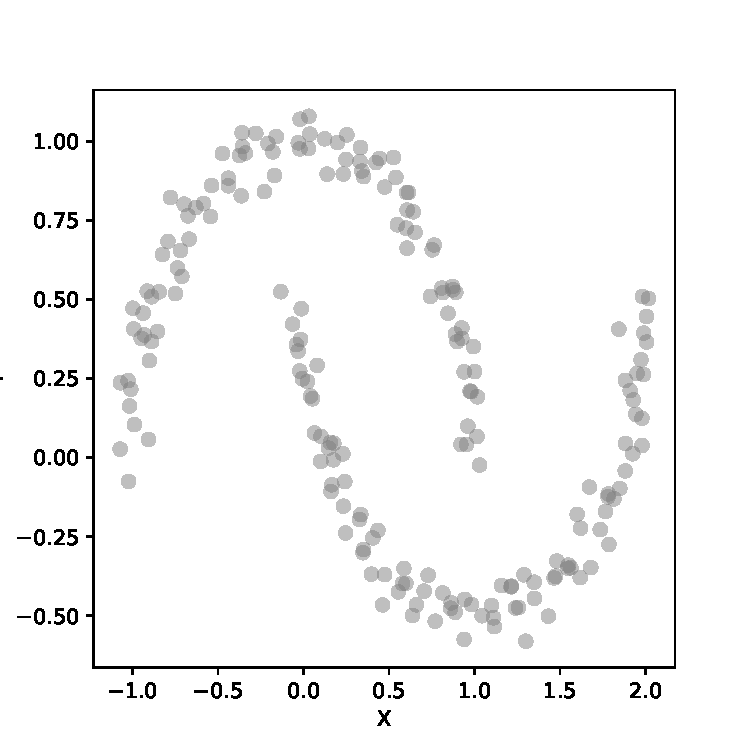
\includegraphics[width=0.5\textwidth]{figures/fake-data.pdf}
    \caption[Datos artificiales]{Datos artificiales en forma de dos lunas para probar los diferentes tipos de agrupaciones.}
    \label{fig:fake-data}

\end{figure}

\subsection{Agrupamiento por K-medias}
El algoritmo de k-medias clasifica los datos separando los datos en $n$ grupos de con la misma varianza.

El algoritmo comienza inicializando aleatoriamente $n$ centroides, siendo $n$ el número de agrupaciones que se le han dicho que realice. Estos centroides serán los centros de las agrupaciones que va a realizar, no tienen por qué pertenecer a los datos, pero sí que están contenidos en su misma dimensión. En cada iteración, el algoritmo asigna a cada punto de los datos el centroide más próximo y luego asigna a cada agrupación un nuevo centroide calculado como la media de los datos que se han asignado a dicha agrupación.

Formalmente, el algoritmo divide un conjunto de $n$ puntos $x$ en $k$ agrupaciones disjuntas $C$, cada una descrita por la media $\mu_j$ de los puntos en la agrupación. Para ello, el algoritmo trata de encontrar los centroides que minimicen

\begin{equation}
  \sum\limits_{i=0}^n \underset{\mu_j \in C}{\operatorname{min}} (|| x_i - \mu_j||^2)
\end{equation}

El algoritmo finaliza cuando una iteración no realice ninguna modificación de las agrupaciones.

\begin{mypython}[float={h},caption={k-medias.}]
    kmeans = KMeans(n_clusters=2, n_init="auto")
kmeans_assigment = kmeans.fit_predict(X)
\end{mypython}

\subsection{Agrupación aglomerada}

\begin{mypython}[float={h},caption={Propagación de afinidad.}]
    agg = AgglomerativeClustering()
    agg_assigment = agg.fit_predict(X)
\end{mypython}

\subsection{Agrupación por afinidad}

El algoritmo de propagación de afinidad crea agrupaciones mandando mensajes entre pares de puntos hasta que converge. La principal cualidad de este algoritmo es que, a diferencia con la mayoría de algoritmos de agrupamiento, no necesita saber el número de agrupaciones a realizar de antemano, sino que las genera dinámicamente.

\begin{mypython}[float={h},caption={Propagación de afinidad.}]
    aff = AffinityPropagation()
    aff_assigment = aff.fit_predict(X)
\end{mypython}

\subsection{Análisis de componentes principales}

\section{Métodos supervisados}
\cite[Deep Learning with PyTorch]{pytorch}
\subsection{Red neuronal}